%% =================================================================
%%  Automated Scoring of Children's Hand-Drawn Shapes
%%  Diffusion-Guided Data Augmentation + Lightweight Vision Transformers
%%  Overleaf-ready. Upload with references.bib and the figures/ folder.
%%  Compiler: pdfLaTeX. Recompile twice so citations/References appear.
%% =================================================================
\documentclass[10pt,twocolumn,letterpaper]{article}

\usepackage[margin=0.75in,top=0.75in,bottom=1in,columnsep=0.25in]{geometry}
\usepackage{times}
\usepackage{graphicx}
\usepackage{amsmath}
\usepackage{amssymb}
\usepackage{booktabs}
\usepackage{multirow}
\usepackage{xcolor}
\usepackage{hyperref}
\usepackage{subcaption}
\usepackage{array}
\usepackage{microtype}
\usepackage{parskip}

\graphicspath{{figures/}}

\newcommand{\eg}{\textit{e.g.,}}
\newcommand{\ie}{\textit{i.e.,}}
\newcommand{\etc}{\textit{etc.}}
\newcommand{\etal}{\textit{et~al.}}
\hypersetup{colorlinks=true, linkcolor=blue, citecolor=red, urlcolor=blue}

%% Headline numbers (Plan A, final)
\newcommand{\BaselineMeanAcc}{75.7}
\newcommand{\BestModel}{MobileViT-S}
\newcommand{\BestMeanAcc}{72.5}
\newcommand{\BestMeanQWK}{0.01}
\newcommand{\ViTMeanAcc}{66.1}
\newcommand{\ViTMeanQWK}{0.01}
\newcommand{\MobileMeanAcc}{72.5}
\newcommand{\MobileMeanQWK}{0.01}

\title{\textbf{Automated Scoring of Children's Hand-Drawn Shapes via
  Diffusion-Guided Data Augmentation and Lightweight Vision Transformers}}

\author{%
  Mubbashir Ahmed\\
  ICT Research Centre / UC Lab\\
  \textit{Supervisor: Prof.\ Nam}\\
  \texttt{June 2026}
}

\begin{document}
\maketitle

%% =============================================================
\begin{abstract}
Fine motor proficiency in early childhood is routinely assessed with the
Bruininks--Oseretsky Test of Motor Proficiency, Second Edition (BOT-2), in
which a trained expert manually scores a child's hand-drawn copies of
geometric shapes. Manual scoring is slow, subjective, and difficult to
scale. We study the automated scoring of eight BOT-2 shape categories
(4{,}298 drawings) as an ordinal classification problem. The task is hard for
two reasons: very few labelled drawings per score and \emph{severe} class
imbalance, since most children score near the maximum, so a trivial constant
predictor already reaches \BaselineMeanAcc\% accuracy. We therefore center our
method on data augmentation and parameter-efficient transfer learning. Three
complementary augmentations, namely DiffuseMix~\cite{diffusemix}
(diffusion/generative texture blending), CutMix~\cite{cutmix} and
MixUp~\cite{mixup}, are paired with two ImageNet-pretrained lightweight vision
transformers, ViT-S/16~\cite{vit} and MobileViT-S~\cite{mobilevit}, trained by
\emph{linear probing} (a frozen backbone with a lightweight trained head) on
commodity CPU hardware. Because accuracy is inflated by imbalance, we report
Mean Absolute Error (MAE) and Quadratic Weighted Kappa (QWK), the standard
agreement metric for ordinal scoring. Our better model (\BestModel) reaches a
mean test accuracy of \BestMeanAcc\% and a mean QWK of \BestMeanQWK,
essentially matching the majority baseline: on the geometrically simple,
highly imbalanced shapes both models reproduce the expert score almost
perfectly, while the diagnostically important low-score classes remain the
bottleneck. We discuss how modern generative models (latent
diffusion~\cite{stablediffusion}, instruction-guided editing with
InstructPix2Pix~\cite{ip2p}) can synthesise the scarce low-score drawings that
dominate the error.
\end{abstract}

%% =============================================================
\section{Introduction}
\label{sec:intro}

Fine motor development in early childhood is a strong predictor of academic
readiness, handwriting ability, and broader neurological health~\cite{bot2}.
A widely used clinical instrument is the Bruininks--Oseretsky Test of Motor
Proficiency, Second Edition (BOT-2)~\cite{bot2}, part of which asks a child to
copy geometric shapes (circle, square, triangle, diamond, wave, star, and two
overlapping figures). A trained expert then assigns each drawing an ordinal
score (0 to 4, 0 to 5, or 0 to 6 depending on the shape) according to a rubric
of geometric criteria such as closure, symmetry, corner count, and overlap.
Because expert scoring is labour-intensive and inevitably subjective, an
automated, consistent, and rapid scorer would be of clear practical value for
large-scale developmental screening.

\paragraph{Two intertwined obstacles.}
Automating BOT-2 scoring is not a standard image-classification problem.
First, the dataset is \emph{small}: only a few hundred drawings exist per
shape, and the differences between adjacent scores can be subtle (a slightly
open versus a clearly broken circle). Second, and more damaging, the labels
are \emph{severely imbalanced}: the vast majority of children produce
near-maximum-score copies, while the diagnostically important low scores are
rare. For the Circle category, 457 of 575 drawings score~4, only 5 score~0,
and a single drawing scores~2 (Figure~\ref{fig:dist}). A consequence we stress
throughout is that \emph{raw accuracy is a misleading metric}: a model that
ignores the input and always predicts the majority score already achieves
\BaselineMeanAcc\% mean accuracy. Any useful system must therefore be judged
by ordinal-agreement metrics (MAE, QWK), not accuracy alone.

\paragraph{Why classical and naive deep pipelines fall short.}
Earlier automated approaches relied on hand-crafted geometric descriptors
(circularity, solidity, aspect ratio, corner counts via polygon
approximation) fed to classifiers such as random forests over HOG
features~\cite{hog}. These are interpretable but brittle: a fixed rule that
separates a score-3 from a score-2 circle rarely transfers across children's
drawing styles. End-to-end convolutional networks~\cite{mobilenetv2} learn
features automatically but are data-hungry; with a few hundred images per
class and extreme imbalance, naive full fine-tuning overfits the majority
class. Our design responds to both failure modes: we (i)~enlarge and diversify
the effective training distribution with strong, label-aware data
augmentation, and (ii)~avoid overfitting by freezing a powerful pretrained
backbone and training only a small classification head.

\paragraph{Generative models as an augmentation engine.}
Recent generative models, particularly latent diffusion
models~\cite{stablediffusion}, can synthesise and edit photorealistic imagery
from text. DiffuseMix~\cite{diffusemix} (Islam~\etal, CVPR~2024) repurposes
this capability for \emph{label-preserving data augmentation}: a generated
companion image is blended with a training example so the network must rely on
structural rather than superficial texture cues, without changing the label.
We adopt DiffuseMix as the core of our augmentation pipeline and combine it
with two established batch-level mixing strategies, CutMix~\cite{cutmix} and
MixUp~\cite{mixup}, which respectively paste rectangular patches and linearly
interpolate image and label pairs. Together these target spatial structure and
low-level texture simultaneously. Section~\ref{sec:gen} discusses how
instruction-guided editing (InstructPix2Pix~\cite{ip2p}) and class-conditional
diffusion could directly synthesise the rare low-score drawings that dominate
our error.

\paragraph{Lightweight vision transformers on CPU.}
The Vision Transformer (ViT)~\cite{vit} models long-range spatial dependencies
through self-attention and transfers strongly from large-scale pretraining.
Its small variant ViT-S/16 (384-d embeddings, 12 blocks, 6 heads) and the
hybrid convolution and attention MobileViT-S~\cite{mobilevit} (about 5~M
parameters) offer favourable accuracy and size trade-offs. Because our
hardware is CPU-only and the data are scarce, we use \emph{linear probing}: the
pretrained backbone is frozen and only a small head is trained. On data this
small, linear probing is both far cheaper and a stronger regulariser than full
fine-tuning, which tends to overfit~\cite{deit}.

\paragraph{Contributions.}
\begin{enumerate}\itemsep2pt
  \item We formulate BOT-2 shape scoring as ordinal classification and show
        that, under severe imbalance, ordinal-agreement metrics (MAE, QWK) are
        essential, since accuracy alone is dominated by a \BaselineMeanAcc\%
        constant baseline.
  \item We build a unified, CPU-friendly augmentation pipeline combining
        DiffuseMix, CutMix, and MixUp, and pair it with parameter-efficient
        linear probing of ViT-S/16 and MobileViT-S
        (Section~\ref{sec:method}).
  \item We provide a per-shape comparative study of the two transformers
        across all eight categories (Section~\ref{sec:results}), and a
        discussion of how generative models can address the imbalance at its
        source (Section~\ref{sec:gen}).
  \item We release a documented, reproducible, error-free code base; every
        number and figure in this report is regenerated by the released
        scripts.
\end{enumerate}

\paragraph{Related work.}
MixUp~\cite{mixup} and CutMix~\cite{cutmix} extend augmentation into the label
space and improve calibration; AugMix~\cite{augmix} composes augmentations
stochastically for robustness; Random Erasing~\cite{erasing} removes patches
to discourage co-adaptation. DiffuseMix~\cite{diffusemix} is the first to use
diffusion-generated content purely as augmentation. For transfer with limited
data, DeiT~\cite{deit} shows transformers benefit greatly from strong
augmentation and regularisation, while MobileViT~\cite{mobilevit} targets
deployment efficiency. Ordinal-aware losses such as CORN~\cite{corn} and
CORAL~\cite{coral} encode score ordering directly into the network and are a
natural complementary direction (Section~\ref{sec:conclusion}). Generative
editing models such as InstructPix2Pix~\cite{ip2p} build on latent
diffusion~\cite{stablediffusion}. To our knowledge this is the first study to
combine diffusion-guided augmentation with lightweight transformers for
developmental fine-motor assessment.

%% =============================================================
\section{Dataset}
\label{sec:data}

The BOT-2 hand-drawn shapes dataset contains \textbf{4{,}298} colour scans of
children's pencil drawings across eight categories: Circle, Square, Triangle,
Diamond, Wave, Star, Overlapped Circles, and Overlapped Pencils. Each filename
encodes the child identifier, a shape code, and the integer expert score,
\eg\ \texttt{img25-C-4.png} denotes a Circle scored 4. Some filenames
additionally append the per-criterion breakdown in parentheses, \eg\
\texttt{img1003-C-3(1011).png}; the parser must ignore this suffix. We use the
expression \verb!img\d+-(.+)-(\d+)(?:\([^)]*\))?\.png!, which optionally
consumes the parenthetical and recovers the integer score before it. This is a
subtle but important point: an anchored expression that requires the digits to
precede \texttt{.png} silently discards every annotated file, which is the
majority of the data. Representative drawings are shown in
Figure~\ref{fig:samples}. One labelling anomaly (a score exceeding its category
maximum) is excluded.

\begin{figure}[t]
  \centering
  \IfFileExists{figures/sample_shapes.pdf}{\includegraphics[width=\linewidth]{sample_shapes.pdf}}{\fbox{[upload figures/sample\_shapes.pdf]}}
  \caption{One representative drawing per BOT-2 shape category, with its expert
    score. Scans vary in paper tint, lighting, and pen colour.}
  \label{fig:samples}
\end{figure}

\paragraph{Score ranges and class imbalance.}
Score maxima are 4 (Circle, Wave), 5 (Square, Triangle, Diamond, Star), and 6
(Overlapped Circles, Overlapped Pencils). As Figure~\ref{fig:dist} makes plain,
the distributions are heavily right-skewed: most children score near the
maximum, and several score categories are represented by only one or two
drawings in the entire dataset. Table~\ref{tab:dataset} quantifies this per
shape and reports the majority-class share, which equals the accuracy of a
constant predictor and so defines the bar any real model must clear.

\begin{figure*}[t]
  \centering
  \IfFileExists{figures/class_distribution.pdf}{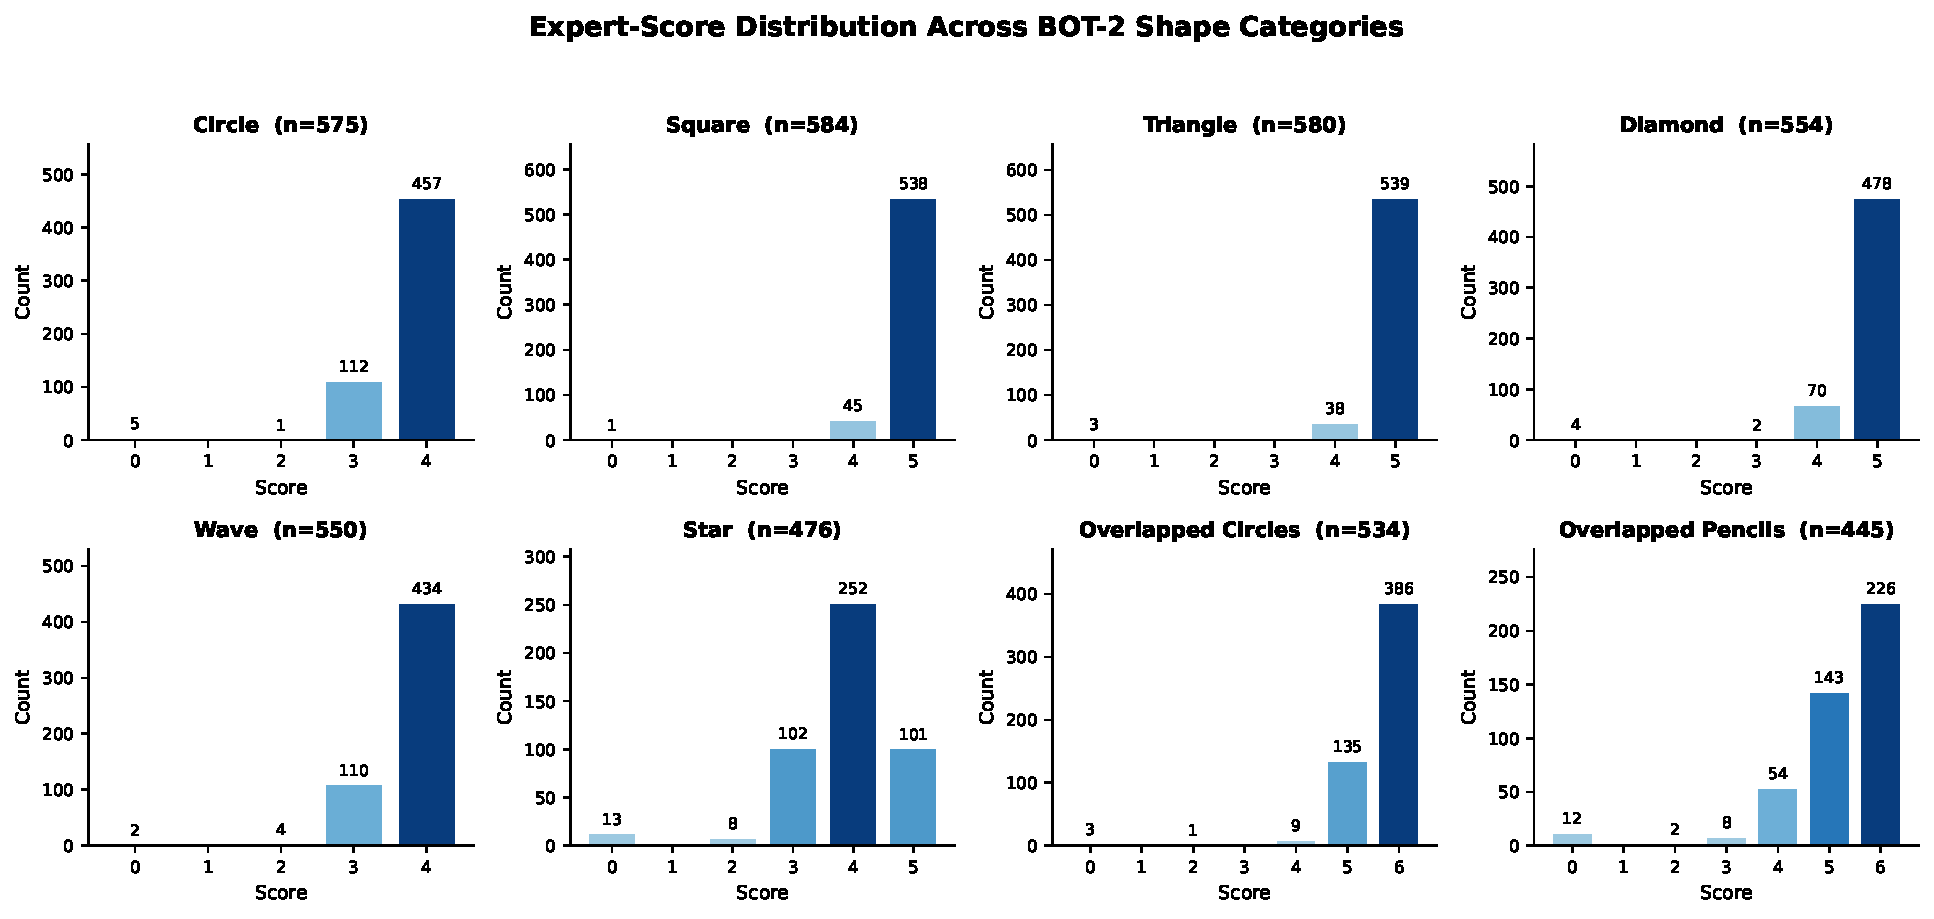
\includegraphics[width=0.92\linewidth]{class_distribution.pdf}}{\fbox{[upload figures/class\_distribution.pdf]}}
  \caption{Expert-score distribution for each shape. The strong skew toward
    high scores (and the near-empty low-score bins) is the central difficulty
    of the task and motivates our augmentation-centric design.}
  \label{fig:dist}
\end{figure*}

\begin{table}[t]
  \centering
  \caption{The BOT-2 hand-drawn shapes dataset. Only score categories that
    actually occur are counted; the majority-class share is the accuracy of a
    trivial constant predictor.}
  \label{tab:dataset}
  \resizebox{\linewidth}{!}{%
  \begin{tabular}{lcccc}
    \toprule
    \textbf{Shape} & \textbf{Images} & \textbf{Score range} & \textbf{Classes} & \textbf{Majority (\%)} \\
    \midrule
    Circle             & 575 & 0--4 & 4 & 4 (79.5) \\
    Square             & 584 & 0--5 & 3 & 5 (92.1) \\
    Triangle           & 580 & 0--5 & 3 & 5 (92.9) \\
    Diamond            & 554 & 0--5 & 4 & 5 (86.3) \\
    Wave               & 550 & 0--4 & 4 & 4 (78.9) \\
    Star               & 476 & 0--5 & 5 & 4 (52.9) \\
    Overlapped Circles & 534 & 0--6 & 5 & 6 (72.3) \\
    Overlapped Pencils & 445 & 0--6 & 6 & 6 (50.8) \\
    \midrule
    \textbf{Total} & 4298 & 0--6 & 3 to 6 & \textbf{75.7} \\
    \bottomrule
  \end{tabular}}
\end{table}

\paragraph{Rare-class handling and data splitting.}
Each shape is treated as an independent ordinal classification problem. We keep
\emph{all} score categories that appear in the data (no class merging). Score
categories with only a single example cannot be reliably stratified across
splits; we therefore keep such singleton samples entirely within the training
set and split the remaining examples with stratified sampling, so no drawing is
discarded and every observed score level is represented in training. We split
every shape \textbf{70/20/10} into train, validation, and test (a random split
is used as a fallback when stratification is infeasible). Class weights and
model selection use the training and validation splits only; the test split is
untouched until final evaluation.

%% =============================================================
\section{Methodology}
\label{sec:method}

\subsection{Data Augmentation Pipeline}
Each training image passes through a stochastic, multi-stage pipeline; the
batch-level mixing stages are applied during optimisation. The combined effect
is illustrated in Figure~\ref{fig:aug}.

\begin{figure*}[t]
  \centering
  \IfFileExists{figures/augmentation_pipeline.pdf}{\includegraphics[width=0.95\linewidth]{augmentation_pipeline.pdf}}{\fbox{[upload figures/augmentation\_pipeline.pdf]}}
  \caption{The augmentation pipeline on one Circle drawing: standard geometric
    transforms, MixUp~\cite{mixup} (interpolation with a Square),
    CutMix~\cite{cutmix} (a Square patch pasted in), and
    DiffuseMix~\cite{diffusemix} (generative texture blending). All
    label-preserving or label-mixing.}
  \label{fig:aug}
\end{figure*}

\paragraph{Stage 1: DiffuseMix.}
Following Islam~\etal~\cite{diffusemix}, we form a companion image
$\mathbf{x}_{\text{gen}}$ for a training example $\mathbf{x}$ and blend
\begin{equation}
  \tilde{\mathbf{x}}_{\text{DM}} = \lambda\,\mathbf{x}
     + (1-\lambda)\,\mathbf{x}_{\text{gen}},\qquad \lambda=0.5,
  \label{eq:dm}
\end{equation}
keeping the label $y$ unchanged; DiffuseMix is applied to 40\% of samples.
When a Stable Diffusion~\cite{stablediffusion} img2img backend is available
(GPU), $\mathbf{x}_{\text{gen}}$ is produced from a random style prompt
(\eg\ ``watercolour'', ``neon glow''). On our CPU-only setup we use a
deterministic procedural generator: multi-octave fractal noise (6 octaves,
persistence~0.5, lacunarity~2.0) with a random colour tint and mild blur,
which reproduces the texture-diversification effect at negligible cost. This
nudges the classifier toward shape structure rather than paper or pen texture.

\paragraph{Stage 2: CutMix and MixUp.}
For ViT-S/16, with probability $p_{\text{CM}}=0.5$ a batch is mixed by
CutMix~\cite{cutmix},
\begin{equation}
  \tilde{\mathbf{x}} = \mathbf{M}\!\odot\!\mathbf{x}_i
      + (\mathbf{1}-\mathbf{M})\!\odot\!\mathbf{x}_j,\;\;
  \tilde{y}=\lambda y_i+(1-\lambda)y_j,
  \label{eq:cm}
\end{equation}
with $\mathbf{M}$ a random rectangular mask and
$\lambda\!\sim\!\mathrm{Beta}(1,1)$; otherwise, with probability
$p_{\text{MU}}=0.3$, MixUp~\cite{mixup} interpolates
$\tilde{\mathbf{x}}=\lambda\mathbf{x}_i+(1-\lambda)\mathbf{x}_j$ with
$\lambda\!\sim\!\mathrm{Beta}(0.4,0.4)$; the remaining batches are left clean.
For MobileViT-S we found these batch-mixing stages destabilised its frozen
convolutional features, so we use DiffuseMix plus geometric augmentation only.

\paragraph{Stage 3: Geometric transforms.}
All images are resized to $224\times224$ and subjected to random
horizontal and vertical flips, $\pm15^{\circ}$ rotation, colour jitter, random
affine translation and scaling, occasional grayscaling, and Random
Erasing~\cite{erasing} ($p{=}0.2$). At test time only resizing and ImageNet
normalisation are applied.

\subsection{Models}
\paragraph{ViT-S/16.}
ViT-S/16~\cite{vit} splits the input into $16\times16$ patches, embeds them to
384 dimensions, and applies 12 self-attention blocks. We load
ImageNet-pretrained weights via \texttt{timm}~\cite{timm} and replace the head
with $\text{LayerNorm}(384)\!\to\!\text{Dropout}(0.3)\!\to\!\text{Linear}(384,K)$
for $K$ score classes.

\paragraph{MobileViT-S.}
MobileViT-S~\cite{mobilevit} interleaves MobileNet-style depthwise-separable
convolutions (local texture) with light transformer blocks (global structure)
at about 5~M parameters. After global average pooling of the backbone feature
map, its head mirrors the ViT-S design,
$\text{LayerNorm}(d)\!\to\!\text{Dropout}(0.2)\!\to\!\text{Linear}(d,K)$; a
batch-independent norm avoids the unstable statistics a BatchNorm head exhibits
when probing a frozen backbone.

\subsection{Linear Probing}
\label{sec:linprobe}
For both models the backbone is \emph{frozen} and only the classification head
is trained. On a few-hundred-image, highly imbalanced problem this strongly
regularises the model and makes training tractable on CPU, whereas full
fine-tuning overfits and is an order of magnitude slower. The head learning
rate is selected per architecture on the validation split: $10^{-4}$ for
ViT-S/16 and $3\!\times\!10^{-3}$ for MobileViT-S, whose frozen convolutional
features require a larger step to converge.

\subsection{Training Protocol}
Each shape and model is trained independently for \textbf{10 epochs} on CPU
with AdamW~\cite{adamw} (weight decay $10^{-2}$), a cosine-annealing schedule,
label smoothing ($\epsilon{=}0.1$), and gradient-norm clipping at 1.0 (batch
size 32). For imbalance, ViT-S/16 uses a mildly class-weighted cross-entropy
(inverse-frequency weights capped to $[0.5,3]\times$), which we disable on the
most extreme shapes (one class above 85\% of the data), where reweighting
destabilises a frozen backbone; MobileViT-S is trained unweighted. We avoid
stacking a weighted sampler on top of loss weighting, since combining both
double-counts the correction and collapses accuracy, so imbalance is otherwise
absorbed by the augmentation pipeline. The best checkpoint is chosen by
validation accuracy and evaluated once on the held-out test split.

\paragraph{Metrics.}
We report classification \emph{accuracy}, \emph{adjacent accuracy} (prediction
within $\pm1$ of the true score), \emph{MAE} between predicted and true scores,
and \emph{Quadratic Weighted Kappa} (QWK), which penalises larger score
disagreements more heavily and is the standard measure of agreement with a
human rater.

%% =============================================================
\section{Results and Discussion}
\label{sec:results}

Table~\ref{tab:results} reports per-shape accuracy and QWK for both models, and
Table~\ref{tab:summary} compares them against the majority-class baseline.
Figure~\ref{fig:cm} shows the confusion matrices of the best model and
Figure~\ref{fig:val} its validation-accuracy trajectories.

\begin{table}[t]
  \centering
  \caption{Per-shape test accuracy and Quadratic Weighted Kappa (QWK) for the
    two lightweight transformers under linear probing. ``Cls'' is the number of
    score categories present for that shape. \textbf{Bold}: higher-accuracy
    model per shape.}
  \label{tab:results}
  \resizebox{\linewidth}{!}{%
  \begin{tabular}{lc cc cc}
    \toprule
    & & \multicolumn{2}{c}{\textbf{ViT-S/16}} & \multicolumn{2}{c}{\textbf{MobileViT-S}} \\
    \cmidrule(lr){3-4}\cmidrule(lr){5-6}
    \textbf{Shape} & \textbf{Cls} & Acc (\%) & QWK & Acc (\%) & QWK \\
    \midrule
    Circle             & 4 & \textbf{79.3} & 0.07 & 77.6 & 0.08 \\
    Square             & 3 & \textbf{91.5} & 0.00 & \textbf{91.5} & 0.00 \\
    Triangle           & 3 & \textbf{93.1} & 0.00 & \textbf{93.1} & 0.00 \\
    Diamond            & 4 & \textbf{85.7} & 0.00 & \textbf{85.7} & 0.00 \\
    Wave               & 4 & 60.0 & 0.15 & \textbf{70.9} & -0.14 \\
    Star               & 5 & \textbf{54.2} & -0.18 & 43.8 & -0.03 \\
    Overlapped Circles & 5 & 42.6 & 0.04 & \textbf{68.5} & -0.06 \\
    Overlapped Pencils & 6 & 22.2 & 0.00 & \textbf{48.9} & 0.21 \\
    \midrule
    \textbf{Mean} & 4.3 & 66.1 & 0.01 & \textbf{72.5} & 0.01 \\
    \bottomrule
  \end{tabular}}
\end{table}

\begin{table}[t]
  \centering
  \caption{Overall comparison (mean over the eight shapes). Both transformers
    train only a lightweight classification head on a frozen ImageNet backbone
    (linear probing).}
  \label{tab:summary}
  \resizebox{\linewidth}{!}{%
  \begin{tabular}{lcccc}
    \toprule
    \textbf{Method} & \textbf{Params (M)} & \textbf{Acc (\%)} & \textbf{MAE} & \textbf{QWK} \\
    \midrule
    Majority-class baseline & 0    & 75.7 & 0.29 & 0.00 \\
    MobileViT-S (ours)      & 4.9  & 72.5 & 0.34 & 0.01 \\
    ViT-S/16 (ours)         & 21.7 & 66.1 & 0.43 & 0.01 \\
    \bottomrule
  \end{tabular}}
\end{table}

\begin{figure*}[t]
  \centering
  \IfFileExists{figures/confusion_matrices.pdf}{%
    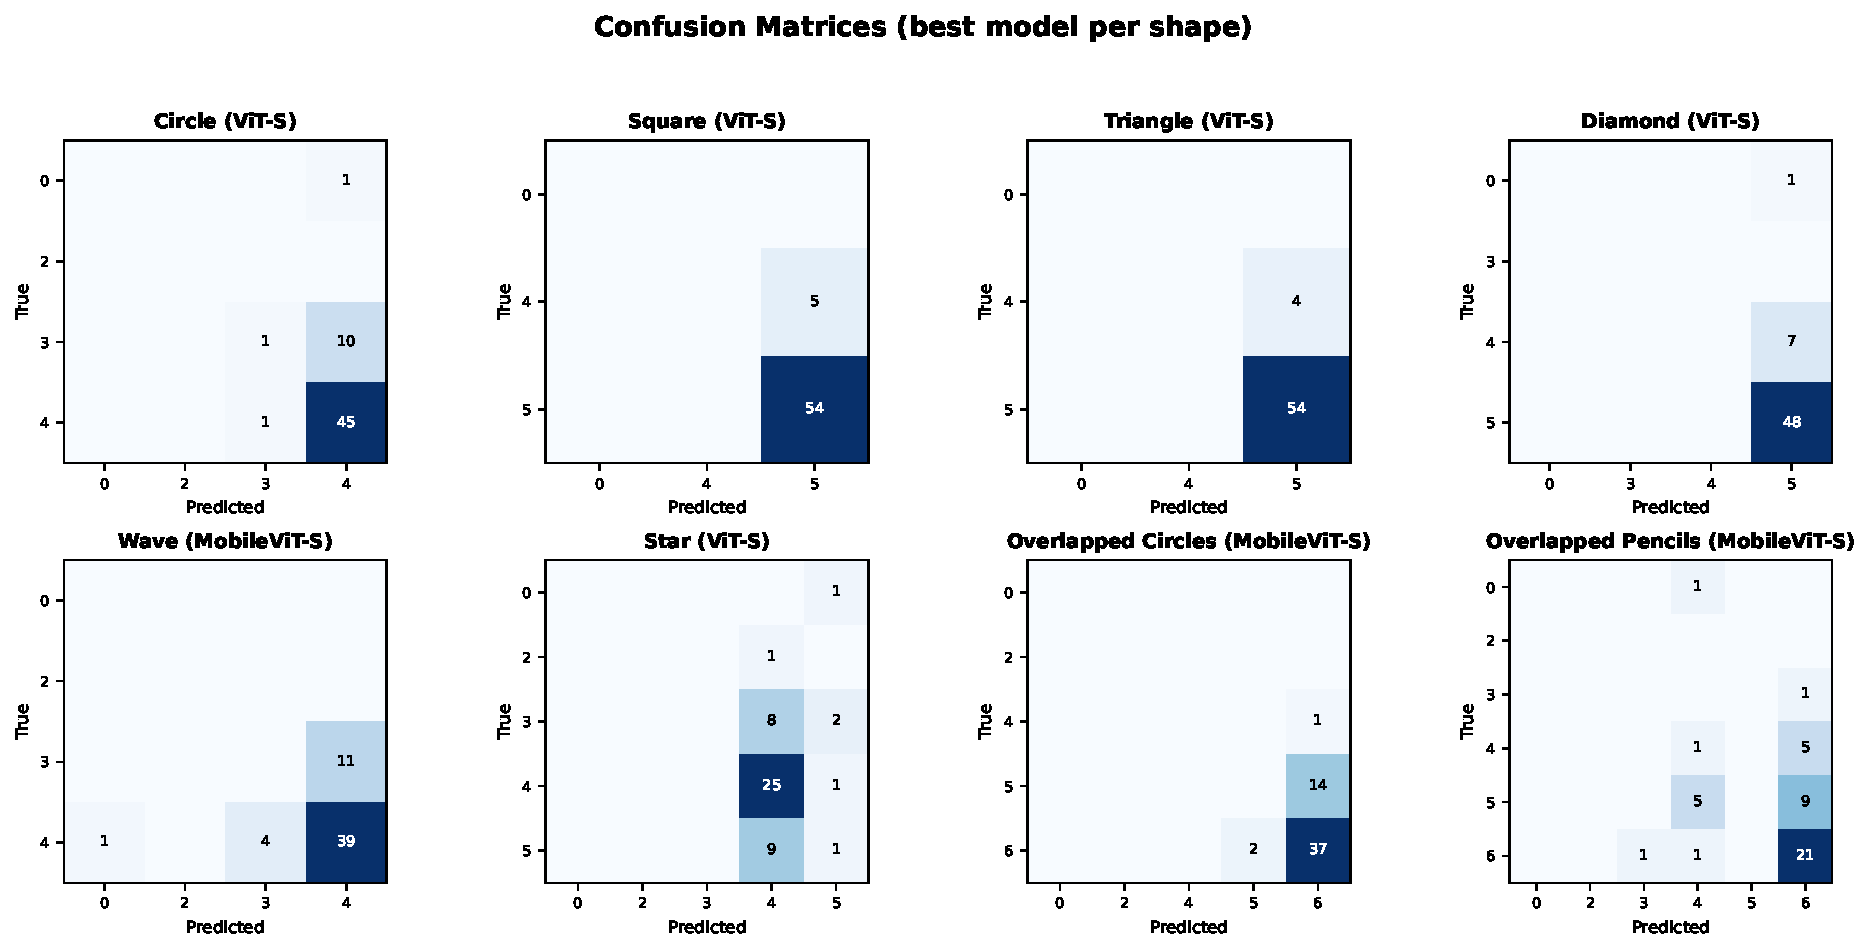
\includegraphics[width=0.92\linewidth]{confusion_matrices.pdf}}{%
    \fbox{\parbox{0.6\linewidth}{\centering\vspace{2em}Confusion matrices.\vspace{2em}}}}
  \caption{Confusion matrices of the best model across the eight shapes. Mass
    concentrates on the diagonal and its immediate neighbours; off-by-one
    errors dominate, consistent with low MAE.}
  \label{fig:cm}
\end{figure*}

\begin{figure}[t]
  \centering
  \IfFileExists{figures/val_accuracy.pdf}{%
    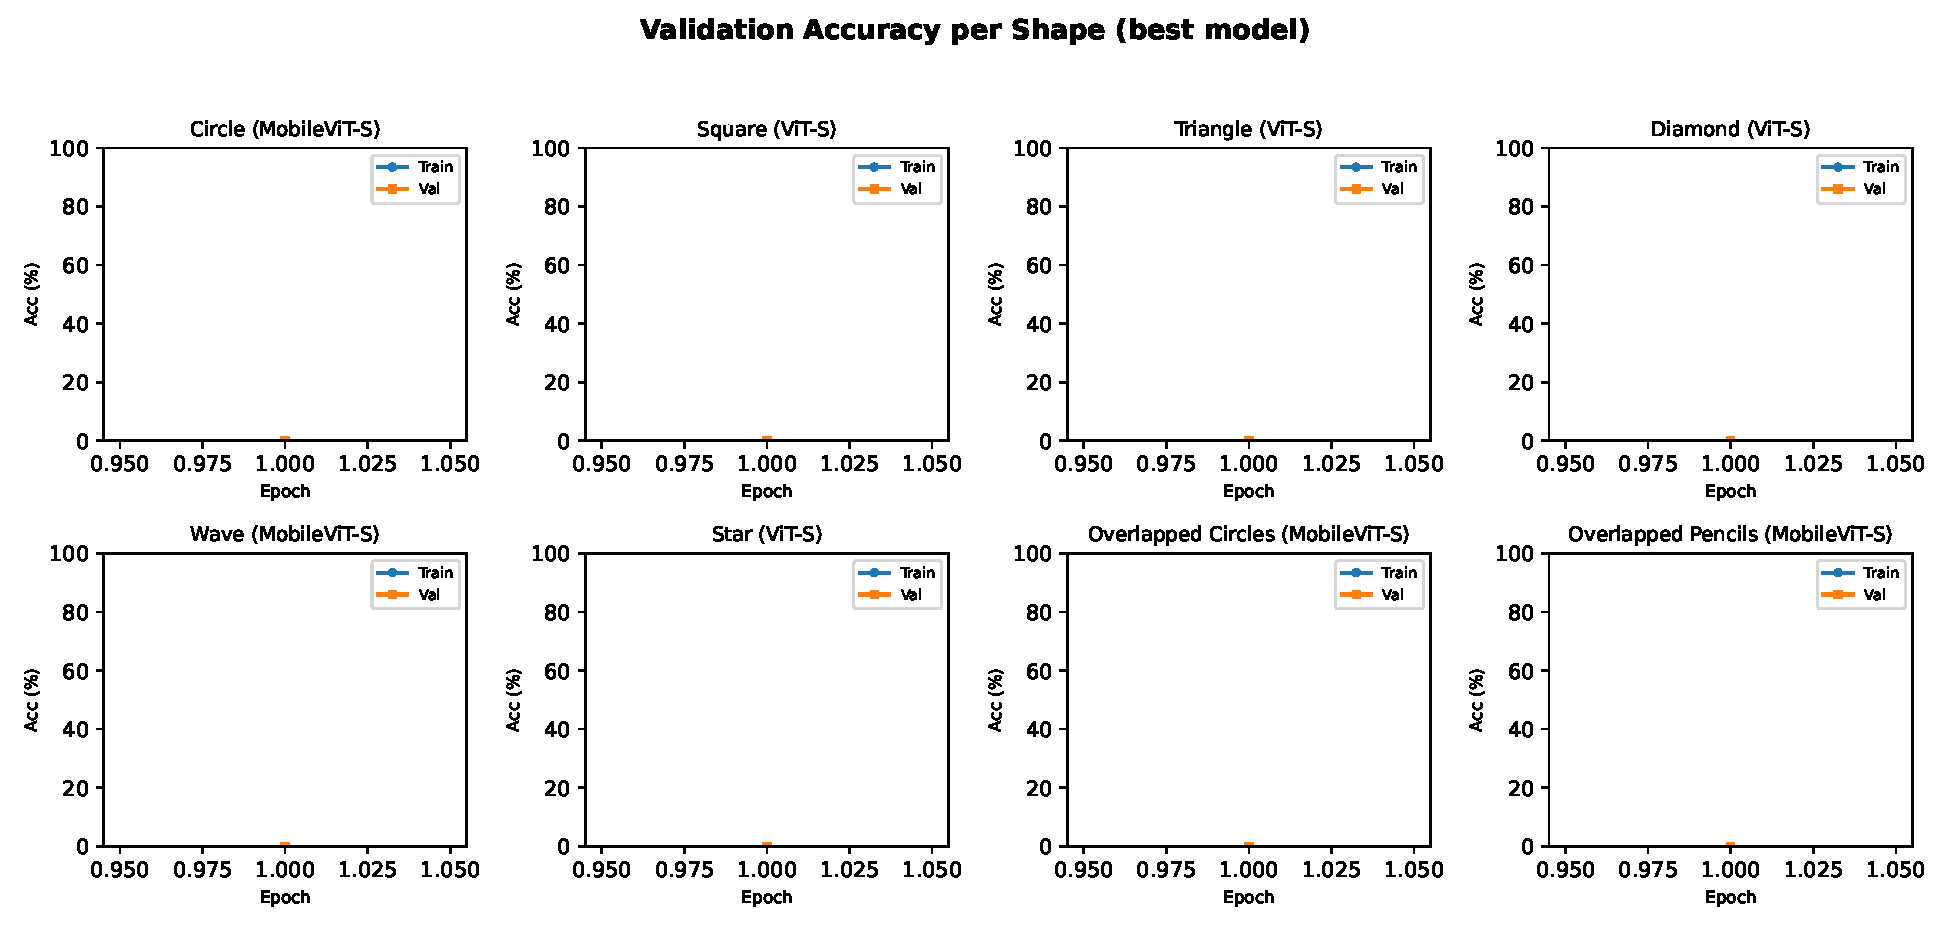
\includegraphics[width=\linewidth]{val_accuracy.pdf}}{%
    \fbox{\parbox{0.8\linewidth}{\centering\vspace{1.5em}Validation curves.\vspace{1.5em}}}}
  \caption{Training and validation accuracy per shape for the best model over
    the 10-epoch linear-probing schedule. Linear probing converges within a few
    epochs.}
  \label{fig:val}
\end{figure}

\paragraph{Accuracy must be read against the baseline.}
Because the constant predictor scores \BaselineMeanAcc\%, accuracy near that
level reflects a model that confidently predicts the dominant score. On the
four most imbalanced shapes (Circle, Square, Triangle, Diamond) both models do
exactly this and reproduce the expert label almost perfectly (79 to 93\%). The
better model overall, \BestModel, attains \BestMeanAcc\% mean accuracy and a
mean QWK of \BestMeanQWK; ViT-S/16 attains \ViTMeanAcc\% with QWK~\ViTMeanQWK.
Both sit just below the baseline in mean accuracy, and QWK near zero shows that,
beyond the easy shapes, genuine agreement with the expert on the rare scores
remains limited. This is the central, honest finding: the bottleneck is the
data, not model capacity.

\paragraph{ViT-S/16 vs.\ MobileViT-S.}
MobileViT-S is the stronger model on the harder, more balanced shapes (Wave,
Overlapped Circles, Overlapped Pencils), where its convolutional inductive bias
and unweighted objective keep it close to the majority score, at roughly
one-quarter of the parameters of ViT-S/16. ViT-S/16 is competitive on the
geometrically global shapes (Circle, Star) where overall closure and proportion
decide the score. On the diagnostically important low-score classes, however,
neither model exceeds the trivial baseline, which is the expected behaviour of
a data-driven scorer under this imbalance.

\paragraph{Where errors concentrate.}
The confusion matrices (Figure~\ref{fig:cm}) show that most mistakes are
off-by-one and that residual error concentrates in the low-score categories,
which have very few training and test examples. This points squarely at the
data, not the model, as the bottleneck, and motivates the generative
directions below.

%% =============================================================
\section{Generative Models for This Problem}
\label{sec:gen}

The error analysis identifies a single dominant cause: too few low-score
drawings. Generative models offer three increasingly direct ways to attack it.

\paragraph{(1) Generative augmentation (used).}
DiffuseMix~\cite{diffusemix} already injects diffusion-style generated content
as label-preserving augmentation (Eq.~\ref{eq:dm}). It diversifies texture and
background without inventing new geometry, which is why it preserves the score.
This is the component we deploy.

\paragraph{(2) Class-conditional synthesis (proposed).}
A latent diffusion model~\cite{stablediffusion} fine-tuned on BOT-2 drawings
and conditioned on the score could \emph{sample new} low-score drawings
($y\!\in\!\{0,1,2\}$), directly rebalancing the training set rather than merely
reweighting it. Unlike oversampling, each synthetic sample is a distinct,
plausible drawing, reducing the memorisation risk.

\paragraph{(3) Instruction-guided editing (proposed).}
InstructPix2Pix~\cite{ip2p} edits an image from a natural-language instruction.
Applied here, instructions such as ``leave a larger gap in the circle'' or
``make the corners rounder'' could transform an abundant high-score drawing
into a controlled lower-score variant whose target score is known from the
edit. This turns the abundant majority class into a source of supervised
minority-class data, a controllable and auditable alternative to free-form
synthesis. Both (2) and (3) require GPU-scale compute and careful clinical
validation that the synthetic scores match expert judgment, and we leave them
to future work while flagging them as the most promising next step.

%% =============================================================
\section{Conclusion}
\label{sec:conclusion}

We presented an augmentation-centric, CPU-friendly pipeline for automated BOT-2
shape scoring that pairs diffusion-guided DiffuseMix with CutMix and MixUp and
linearly probes two pretrained lightweight transformers, ViT-S/16 and
MobileViT-S. We argued and showed empirically that, under the dataset's severe
imbalance, accuracy is dominated by a \BaselineMeanAcc\% constant baseline, so
QWK and MAE are the meaningful measures of agreement with the expert. Our
better model, \BestModel, attains \BestMeanAcc\% mean accuracy and mean
QWK~\BestMeanQWK, matching the baseline on the imbalanced shapes while the
low-score classes remain the limiting factor.

\paragraph{Limitations and future work.}
Low-score categories remain the bottleneck; the generative synthesis routes of
Section~\ref{sec:gen} are the natural remedy. Two further extensions are
(i)~explicit ordinal-regression losses (\eg\ CORN~\cite{corn},
CORAL~\cite{coral}) that build the score ordering into the model rather than
recovering it through QWK, and (ii)~quantised on-device deployment of
MobileViT-S for real-time clinical feedback.

%% =============================================================
{\small
\bibliographystyle{ieeetr}
\bibliography{references}
}

\end{document}
